\documentclass[12pt,fleqn]{article}\usepackage{../../common}
\begin{document}
Ders 4

Dışbükeylik (Convexity) ve Koniler (Cones) 

Bir lineer vektör uzayındaki $K$ kümesi dişbukeydir (convex), eğer 
$x_1,x_2 \in K$ için $\alpha x_1 + (1-\alpha)x_2$, $0 \le \alpha \le 1$ formundaki
tüm noktalar da $K$ içinde ise.

Matematiksel olarak $\alpha,1-\alpha$ ile yapılmaya uğraşılan $x_1,x_2$
``arasındaki'' bir noktayı temsil etmek. Eğer $0 \le \alpha \le 1$ ise,
$x_1,x_2$'yi sırasıyla $\alpha,1-\alpha$ ile çarpıp sonuçları toplamak
``biraz $x_1$'den, biraz $x_2$'den almak'' anlamına geliyor, bu da tanım
itibariyle her zaman $x_1,x_2$ arasında bir yerde olmaktır. $\alpha$ 0 ile
1 arasındadır, yani bir nevi yüzde hesabı yapılıyor, 0.2 oradan, 0.8
şuradan alınıyor. Hesabın bir tür yüzde hesabı olması sebebiyle iki nokta
arasında kalınması garanti edilmiş oluyor. 

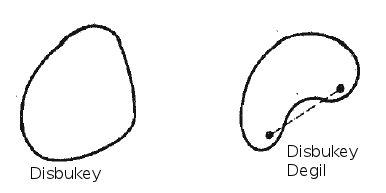
\includegraphics[height=3cm]{4_1.png}

Ve eğer bu ``arada olmak'' denklemi, kümedeki her noktanın her diğer
noktayla arasındaki, yani her $\alpha$ için hesaplanacak noktalar için de
doğru ise, o zaman hep aynı kümedeyi, ``dışarı çıkmıyoruz'' demektir ve bu
dişbukeyliğin tanımıdır. Görsel olarak ta kabaca bunu görmek mümkündür,
dişbukey bir cisimde bir noktadan diğerine düz çizgide giderken hep cisim
içinde kalırız.

Teori 

$K.G$ bir vektör uzayında dışbükey olan iki küme olsun. O zaman 

1. $\alpha K = \{x: x = \alpha k, k \in K\}$ her $\alpha$ için dışbükeydir. 

2. $K+G$ dışbükeydir. 

İspatlamadan bunun daha genel bir hali olan başka bir teoriye bakalım, onu
ispatlarsak üsttekini de ispatlamış olacağız. 

Teori 

$\mathscr{C}$, içindeki tüm kümeleri dışbükey olan rasgele bir buket
olsun. O zaman $\cap_{K \in \mathscr{C}}K$ aynı şekilde dişbukeydir. 

Ispat

Diyelim ki $C = \cap_{K \in \mathscr{C}}K$. Eğer $C$ boş ise, teori hemen
ispatlamıştır. Diğer şartlar için, farzedelim ki $x_1,x_2 \in C$. O zaman
$x_1,x_2 \in K$ demektir, çünkü $C$ bir kesişim, yani tüm $K \in \mathscr{C}$
içindeki aynı olan öğelerden müteşekkil. Her $K$'nin kendi başına dışbükey
olduğunu bildiğimize göre, o zaman $C$ de dışbükey demektir. 

$ \square $

Norm Edilmiş Lineer Uzaylar

Soyut Analiz ve uygulamalarda ilgilenilen vektör uzaylarının 7 önşarttan
daha fazlasına ihtiyacı vardır. 7 önşart vektör uzaylarının sadece cebirsel
özelliklerini tanımlar: toplam, skalar çarpım, ve bunların değişik
kombinasyonları. Eksik olanlar topolojik olan özelliklerdir, yani açıklık
(openness), kapalılık (closure), yakınsaklık (convergence), ve bütünlük
(completeness). Eğer uzayın içinde uzaklık ölçümü tanımlanır ise, bu
kavramlar kullanılabilir. 

Tanım

Norm edilmiş bir lineer uzay $X$ adındaki bir vektör uzayıdır, ki $X$
içindeki her $x$ öğesini bir reel sayı $||x||$'e eşleyen bir fonksiyon
vardır, ve $||x||$'e $x$'in norm'ü adı verilir. Norm şu önşartları yerine
getirmelidir. 

1. $||x|| > 0$, her $x \in X$ için, ve $||x|| = 0$, sadece ve sadece $x =
\theta$ ise. 

2. $||x+y|| \le ||x|| + ||y||$ her $x,y \in X$ için (üçgensel eşitsizlik) 

3. $||\alpha x|| = |\alpha| \ ||x||$, her skalar $\alpha$ ve her $x \in X$ için. 

Norm kavramı uzaklık kavramının soyutlaştırılmış bir halinden ibaret
aslında. Reel analizdeki üçgensel eşitsizliğin karşılığı burada da
görülüyor mesela. Neyse, devam edelim, üstteki üçgensel eşitsizlik
kuralının bir uzantısı / sonucu (lemma) şu:

Teori 

Norm edilmiş bir lineer uzayda 

$$ ||x|| - ||y|| \le ||x-y|| 
\mlabel{1}
$$

İspat

$$ ||x|| - ||y|| = ||x - y + y|| - ||y||$$

Üstte adece $||x||$ içine $-y+y$ ekliyoruz, yani aslında hiçbir şey
değiştirmedik. Şimdi eşitliğin sağındaki ilk terimi alıp ona üçgensel
eşitliği uygularsak (norm içindeki $+$ işareti solu ve sağındaki grupları
ayrı terimler olarak kabul etmemiz gerekir)

$$ ||x - y + y|| - ||y|| \le
||x - y || + ||y|| - ||y|| 
$$

elde ederiz. Biraz daha basitleştirince

$$ ||x|| - ||y||  \le ||x - y ||  $$

$\square$

Uygun bir norm bulunabilirse, daha önce gösterdiğimiz vektör uzayı
örneklerinin çoğunluğu norm edilebilen uzaya dönüştürülebilir.

Örnek 1

$C[a,b]$ adı verilen norm edilmiş uzay, $[a,b]$ reel aralığı, artı norm

$$ ||x|| = \max_{a \le t \le b} |x(t)| $$

tanımından oluşur. Hatırlarsak bu uzay daha önce bir vektör uzayı olarak
gösterilmişti. Norm $[a,b]$ aralığına bakıyor, her $x(t)$ için mutlak değeri
(absolute value) en yüksek olan değeri alıp onu norm değeri ilan
ediyor. Fonksiyon bir parabol ise, parabolun tepe noktası o fonksiyon için
norm kabul edilecek. 

Şimdi teklif edilen norm'un 3 gerekli önşartı yerine getirip getirmediğine
bakalım. Bariz ki $||x|| \ge 0$ çünkü norm kesin değer kullandık ve kesin
değerler hep sıfırdan büyük, ayrıca $||x||$ sıfır olması için $x(t)$'nin
her yerde sıfır olması lazım, fonksiyon tek bir noktada sıfırdan azıcık
daha büyük olsaydı, $max$ hemen onu norm kabul ederdi. Üçgensel eşitsizlik
alttaki ilişkinin bir uzantısı zaten

$$ 
\max |x(t) + y(t)| \le 
\max [|x(t)| + |y(t)|] \le
\max |x(t)| + max |y(t)|
$$

Üstteki eşitsizlikler maksimum fonksiyonun özellikleri, ve bu özellikler
onun üçgensel eşitsizliği de yerine getirmesini sağlıyor. 

En son olarak 3. önşart alttaki ilişkinin doğal sonucu olarak yerine
getirilmiş oluyor 

$$ \max |\alpha x(t)|  = \max |\alpha||x(t)| = |\alpha| \max |x(t)|  $$

Örnek

$[a,b]$ aralığında tanımlı tüm sürekli fonksiyonların uzayı alttaki norm
üzerinden bir norm edilmiş uzaydır

$$ ||x|| = \int _{ a}^{b} |x(t)| \ud t $$

Dikkat, bu norm edilmiş uzay $C[a,b]$'den farklıdır. 

Örnek 

Öklitsel n-uzayı ki $E^n$ olarak temsil edilir, ve norm'u $x = \{ \xi_1,
\xi_2, .., \xi_n\}$ için $||x|| = (\sum _{ i=1}^{n} |\xi_i|^2)^{1/2}$, bir
norm edilmiş uzaydır.

Yakınsaklık (Convergence)

Çoğu zaman, istenen bir özelliğe sahip olan bir vektörün varlığını ispat
ederken belli bir limite yaklaşan bir vektör dizisi yaratmak yaygın bir
tekniktir. Çoğu zaman bu limitin istenen özelliğe sahip olduğu
gösterilebilir. Bu sebeple yakınsaklık (convergence) kavramı Analizde çok
önemli rol oynayan bir kavramdır.

Tanım 

Norm edilmiş bir lineer uzayda sonsuz sayıda vektör içeren bir dizi
$\{x_n\}$'in $x$'e {\em yaklaştığı} söylenir eğer $\{||x_n-x||\}$ reel
sayılar dizisi sıfıra yaklaşıyorsa. Bu durumda $x_n \to x$ diyebiliriz.

Eğer $x_n \to x$, $||x_n|| \to ||x||$ olmalı, çünkü (1)'e göre 

$$ ||x_n||  - ||x|| \le ||x_n-x|| $$

ya da, terimlerin yeri değiştirilmiş halde

$$ ||x||  - ||x_n|| \le ||x-x_n|| $$

O zaman 

$$ \bigg| ||x||  - ||x_n|| \bigg|  \le ||x-x_n|| \to 0$$

olmalıdır. 

Teori 

Eğer bir dizi yaklaşıyorsa, limiti özgündür (unique).

İspat

Diyelim ki $x_n \to x$ ve $x_n \to y$, yani $x_n$ apayrı iki limite
yaklaşıyor (gibi) bir şey ortaya attık. Peki o zaman $||x-y||$ ne olur?
Göreceğiz ki bu norm sıfıra gidecek ve bu sebeple $x,y$'nin birbirinden
farklı olamayacağını anlamış olacağız. 

$$ ||x-y|| =  ||x-x_n + x_n-y|| $$

Üstte yine aynı numarayı kullandık, $-x_n+x_n$ ekleyerek eşitlikte hiçbir
şey değiştirmiyoruz, ama daha fazla terim elde ederek şimdi üçgensel
eşitsizliği kullanabileceğiz. $+$ işaretinin solundaki ve sağındaki
blokları ayrı terimler gibi kabul edersek, 

$$ ||x-x_n + x_n-y|| \le ||x-x_n || + ||x_n-y|| $$

ve

$$ ||x-x_n || \to 0 $$

$$ ||x_n-y|| \to 0$$

olduğuna göre 

$$  ||x-y|| \to 0 $$ 

$\square$

\end{document}
